\documentclass[11pt]{article}
% Paper A --- measurement. Compile: tectonic paper.tex
% Speculation/engine follow-on is not this PDF (umax v2 first).
% Separate from paper/paper.tex (training-time locality, arXiv 2608.18261).
% Every decode number traces to measurements/*verdict.json.
% Do not cite 0.44 tok/s as this CPU stream stack.
\usepackage[margin=1in]{geometry}
\usepackage{amsmath,amssymb}
\usepackage{booktabs}
\usepackage{graphicx}
\usepackage{xcolor}
\usepackage{tikz}
\usepackage{pgfplots}
\pgfplotsset{compat=1.17}
\usepackage{caption}
\usepackage{subcaption}
\usepackage{hyperref}
\hypersetup{colorlinks=true,linkcolor=blue!55!black,citecolor=blue!55!black,urlcolor=blue!55!black}
\usepackage{natbib}
\bibliographystyle{plainnat}

\definecolor{acc}{HTML}{3B6FD0}
\definecolor{wall}{HTML}{B5423A}
\definecolor{ok}{HTML}{2F9E8F}

\newcommand{\tps}{tok/s}

\title{\textbf{Capacity-Law Serving of a 235B Mixture-of-Experts Model\\
on 32\,GB Host Memory}\\[4pt]
\large Routing Traces and Union Demand on a Consumer SSD}
\author{Shriniwas Ramesh Suram\thanks{ORCID: \href{https://orcid.org/0009-0009-0452-9407}{0009-0009-0452-9407}. Work conducted independently on personal hardware (RTX 3070 left idle).}\\
University of Cumberlands, Williamsburg, USA\\
\texttt{ssuram36954@ucumberlands.edu}}
\date{August 2026}

\begin{document}
\maketitle

\begin{abstract}
Qwen3-235B-A22B stores 235B parameters and activates about 22B per token
\citep{yang2025qwen3}. In 4-bit GGUF form the checkpoint is 133\,GB---larger
than a 32\,GB desktop's RAM. We serve it on one Windows/WSL2 workstation
(RTX~3070 8\,GB idle; CPU-only llama.cpp) by streaming MoE experts from NVMe
with \texttt{O\_DIRECT}. Random 3.5/10/16\,MB \texttt{O\_DIRECT} QD8 reads on
the ext4 VHDX measure 2.34--2.37\,GB/s. CPU decode with an 8-slot expert cache
is 0.29\,\tps{}; a 12-slot cache that still fits in 21\,Gi of WSL RAM reaches
0.38\,\tps{} (peak RSS 16.70\,GiB). Full CPU mmap dies allocating a 105\,GB
\texttt{CPU\_REPACK} buffer.

We release 94-layer top-8 routing traces ($4\times 2048$ tokens). Mean unique
experts over a 4-token window is $U(4)=18.98$, so mean unique demand exceeds
16 slots (naive $k{=}4$ still fits 23\% of 16-slot windows).
Identical lag-1 expert \emph{sets} occur 0.26\% of the time; an 8-slot
admission cap has mean admitted length $T{=}1.003$. Causal lag-2 prefetch
recovers 0\% of the LRU--OPT gap on these traces. Per-layer-mean oracle
admission at 12 slots gives $T{=}1.54$ for $k{=}2$; the engine-relevant
aggregate is the \emph{minimum} over 94 layers, $T{=}1.001$
($p(T{\ge}2){=}0.12\%$). This paper measures that geometry. Engine work that
tries to speculate under the law is a separate manuscript.
\end{abstract}

\section{Introduction}
\label{sec:intro}

Mixture-of-Experts (MoE) layers route each token to a top-$k$ subset of
experts \citep{shazeer2017moe,fedus2022switch}. That sparsity is why a
235B-total / 22B-active model \citep{yang2025qwen3} can run at all on a
workstation, but ``runs'' is not ``interactive.'' Offloading Mixtral-8$\times$7B
with an LRU expert cache has been shown to reach 2--3\,\tps{} on a T4, RTX
3060, or RTX 3080 Mobile \citep{eliseev2023mixtraloffload}; MoE-Infinity reports 3.1--16.7$\times$
latency reduction from expert-level traces on a commodity GPU
\citep{xue2024moeinfinity}. Those results do not transfer to a 133\,GB
Qwen3-235B table on 21\,Gi of WSL RAM.

This paper is a \emph{measurement} study of that geometry. Direct I/O streaming
of expert slabs is the substrate (llama.cpp PR\#25294); we do not claim it as a
novelty. The systems question we can answer now is how many \emph{unique}
experts a $k$-token window demands, and whether that union fits in a RAM-sized
slot budget---a \emph{capacity law}, not a bandwidth slogan. Speculative
decoding \citep{leviathan2023speculative} is why the union matters: verify is
cheap only if $U(k)\le s$. We do not report a speculation speedup here.

\paragraph{Contributions.}
\begin{enumerate}\itemsep2pt
\item \textbf{A CPU tok/s ladder on one box} with provenance files: mmap
impossible; 8-slot stream-direct 0.29\,\tps{}; 12-slot 0.38\,\tps{} at 16.70\,GiB RSS.
\item \textbf{235B routing traces} of shape $(94,2048,8)$ on four domains, and the
union law $U(k)$ that falsifies ``just speculate with $k{=}4$.''
\item \textbf{Negatives on the traces:} $U(4)\le 16$ fails; causal prefetch
recovery $W{=}0$; 8-slot HorizonSpec mean admitted length $T{=}1.003$;
engine-min $T{=}1.001$ at 12 slots $k{=}2$.
\end{enumerate}

A 0.44\,\tps{} figure from Windows \texttt{llama-server -ngl 99 -ncmoe 94}
(GPU non-MoE trunk, 2026-08-05) is a \emph{different stack} and is not used
below. The companion training-time locality paper
\citep{suram2026cacheable} pre-registers 137M MoE routers with a locality
loss: cache misses fall up to 60\%, but every configuration fails a
$\le 1\%$ perplexity gate. We do not mix that result---or that paper's
0.44\,\tps{} warm 235B decode---into these CPU stream tables.

\section{Background}
\label{sec:bg}

\paragraph{MoE serving.}
At decode, each token's active experts must be present in a fast tier.
EdgeMoE adapts expert bitwidth and keeps hot experts in an on-device buffer
\citep{yi2023edgemoe}. PowerInfer pins high-frequency neurons on GPU
\citep{song2024powerinfer}. Fiddler runs uncompressed Mixtral-8$\times$7B by
executing CPU-resident experts on the CPU \citep{kamahori2025fiddler}. FlexGen
runs OPT-175B on a single 16\,GB GPU at 1\,\tps{} generation \emph{throughput}
(effective batch size 144), not single-stream decode
\citep{sheng2023flexgen}. Pre-gated MoE prefetches the next block's experts
from the current block's gate \citep{hwang2023pregated}. None of these papers
report Qwen3-235B-A22B top-8 unions on a 12-slot, 21\,Gi CPU stream cache.

\paragraph{Capacity law.}
Let $s$ be the number of expert slots per MoE layer that fit in RAM, $k$ the
lookahead window, and $U(k)$ the number of unique experts in a $k$-token window
at one layer. Greedy decode always loads $U(1)=\mathrm{top}\text{-}8=8$ experts per
layer. A $k$-token step is one I/O generation only if $U(k)\le s$. If an engine
instead instantiates a worst-case graph of $k\times 8$ experts, extra waves pay
compute and I/O even when the realized union is small.
Admission-time $U_{\max}{=}s$ would truncate a prefix so the union fits. On
traces we simulate longest-prefix admission with \emph{target} routing (an upper
bound on sharing). That table is not tok/s.

\section{Setup}
\label{sec:setup}

\paragraph{Machine.}
Windows 11 + WSL2 Ubuntu, Intel i9-12900 (16C/24T), RTX 3070 8\,GB idle,
$\sim$32\,GB host RAM, \texttt{.wslconfig} 22\,GB (WSL \texttt{free}
$\approx$ 21\,Gi), NVMe. llama.cpp branch \texttt{pr-25294}, git
\texttt{1248fd8fa}, \texttt{GGML\_CUDA=OFF}. Model:
\texttt{Qwen3-235B-A22B-Q4\_K\_M} (3-way split, 133\,GB) on ext4. Expert cache
\texttt{--moe-stream-direct --moe-stream-cache \{8s,12s\}}. Context 512,
temperature 0, seed 1. Every headline number has a \texttt{config.json} /
\texttt{verdict.json} under \texttt{measurements/} (Appendix~\ref{app:prov}).

\paragraph{I/O.}
fio 3.39, 20\,s, 30B GGUF on the same VHDX (\texttt{measurements/fio\_summary.tsv}):
mmap QD1 10\,MB ${=}0.064$\,GB/s; \texttt{pread} QD1 ${=}1.377$;
\texttt{O\_DIRECT} QD1 ${=}1.856$; \texttt{O\_DIRECT} QD8 at 3.5/10/16\,MB
${=}2.368/2.339/2.354$\,GB/s.

\paragraph{30B check.}
Same binary, Qwen3-30B-A3B Q4\_K\_M: mmap 1.71\,\tps{} vs stream-direct
3.41\,\tps{} ($1.99\times$). Direct I/O is not a no-op on this host.

\section{The expert table versus the RAM slab}
\label{sec:slab}

Qwen3-235B-A22B uses 94 MoE layers, 128 experts, top-8. At Q4\_K\_M an expert
slab is $10.85$\,MB (\texttt{measurements/uk\_umax\_235b.json}). Greedy decode therefore
demands $94\times 8\times 10.85\,\mathrm{MB}=7.97$\,GB of expert bytes per token
before cache hits. A 12-slot cache is
$12\times 94\times 10.85\,\mathrm{MB}=11.96$\,GB of expert RAM; measured peak
RSS is 16.70\,GiB including activations and the dense trunk
(\texttt{measurements/ab235b\_12s\_verdict.json}). Sixteen slots would add
$\sim$4\,GiB on top of 16.7\,GiB and were not attempted. Full mmap failed:
\texttt{ggml\_aligned\_malloc} of 105\,496\,MB for \texttt{CPU\_REPACK}.

Feasibility is \emph{expert-table bytes divided by RAM slab}, not parameter
count. DeepSeek-V3 is 671B total with 37B activated per token
\citep{deepseekai2024deepseekv3}; a 4-bit table for that geometry is larger
than this 133\,GB Qwen3 checkpoint. We do not claim it is a smooth fit here.

\section{Routing traces and the union law}
\label{sec:traces}

\texttt{llama-moe-trace} records top-8 ids with weights untouched (stream-direct,
8-slot cache, 2048 tokens $\times$ 4 domains, window 512). Shape $(94,2048,8)$.
Provenance: \texttt{measurements/traces/} and \texttt{measurements/uk\_235b.json}.

\begin{table}[t]\centering
\caption{Unique experts $U(k)$ and lag-1 set reuse on Qwen3-235B-A22B top-8
traces. $U(4)\le 16$ fails on every domain. Source:
\texttt{measurements/uk\_235b.json}.}
\label{tab:uk}
\small
\begin{tabular}{lrrrr}
\toprule
domain & $U(4)$ & $U(4)/32$ & lag-1 reuse / chance & ratio \\
\midrule
code     & 18.35 & 0.573 & 0.479 / 0.256 & 1.87$\times$ \\
general  & 18.87 & 0.590 & 0.463 / 0.203 & 2.27$\times$ \\
math     & 20.00 & 0.625 & 0.406 / 0.186 & 2.19$\times$ \\
medical  & 18.71 & 0.585 & 0.459 / 0.236 & 1.95$\times$ \\
\textbf{mean} & \textbf{18.98} & 0.59 & --- & $\sim$2.1$\times$ \\
\bottomrule
\end{tabular}
\end{table}

\begin{figure}[t]
\centering
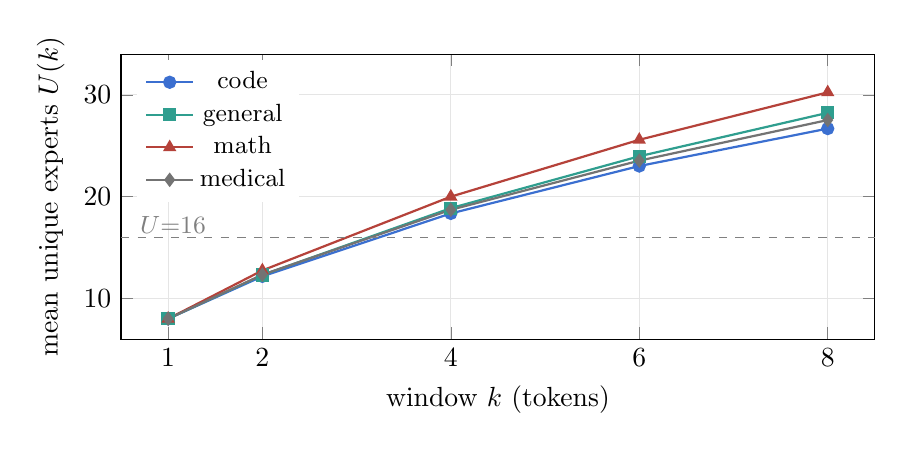
\begin{tikzpicture}
\begin{axis}[
  width=0.92\linewidth, height=5.2cm,
  xlabel={window $k$ (tokens)},
  ylabel={mean unique experts $U(k)$},
  xmin=0.5, xmax=8.5, ymin=6, ymax=34,
  xtick={1,2,4,6,8},
  legend style={font=\small, at={(0.02,0.98)}, anchor=north west, draw=none},
  grid=major, grid style={gray!20},
]
\addplot[color=acc, mark=*, thick] coordinates {(1,8) (2,12.17) (4,18.35) (6,23.01) (8,26.69)};
\addlegendentry{code}
\addplot[color=ok, mark=square*, thick] coordinates {(1,8) (2,12.30) (4,18.87) (6,23.97) (8,28.24)};
\addlegendentry{general}
\addplot[color=wall, mark=triangle*, thick] coordinates {(1,8) (2,12.75) (4,20.00) (6,25.59) (8,30.25)};
\addlegendentry{math}
\addplot[color=black!55, mark=diamond*, thick] coordinates {(1,8) (2,12.33) (4,18.71) (6,23.54) (8,27.53)};
\addlegendentry{medical}
\draw[dashed, gray] (axis cs:0.5,16) -- (axis cs:8.5,16);
\node[gray, font=\small, anchor=west] at (axis cs:0.6,17.2) {$U{=}16$};
\end{axis}
\end{tikzpicture}
\caption{$U(k)$ grows through 16 by $k{=}4$ on every domain
(\texttt{measurements/uk\_235b.json}). Mean $U(4)=18.98$ exceeds 16 slots; naive
$k{=}4$ still fits 23\% of 16-slot windows.}
\label{fig:uk}
\end{figure}

Union sharing is real ($U(4)/32\approx 0.59$) but the union is larger than 16.
Code $U(2)=12.17$: mean unique experts over two tokens \emph{exceeds} 12
slots. Naive $k{=}2$ fits 54\% of 12-slot windows \emph{per layer} (mean over
layers), not a 4-token union and not the minimum over 94 layers.

\section{HorizonSpec is a slot count}
\label{sec:hs}

Longest-prefix admission on these traces (target-oracle routing, an upper
bound on union sharing) gives mean admitted length $T$. Consecutive tokens
share an \emph{identical} 8-expert set 0.26\% of the time
(\texttt{measurements/uk\_umax\_235b.json} pooled). With top-8 routing,
$U_{\max}{=}8$ almost never admits a second token. Mean $T$ at 8 slots is
1.003---greedy.

\begin{table}[t]\centering
\caption{Target-oracle HorizonSpec on 235B traces. Per-layer mean, then mean
over four domains. Not engine $\min$ over layers, not tok/s.
Source: \texttt{measurements/uk\_umax\_235b.json}.}
\label{tab:hs}
\small
\begin{tabular}{lcccc}
\toprule
cap & naive $k{=}2$ fit & HSpec $k{=}2$ $T$ & naive $k{=}4$ fit & HSpec $k{=}4$ $T$ \\
\midrule
8 slots  & 0.26\% & 1.003 & $\sim$0\% & 1.003 \\
12 slots & 54.3\% & 1.54  & 1.2\% & 1.64 \\
16 slots & 100\%  & 2.00  & 23.0\% & 2.83 \\
24 slots & 100\%  & 2.00  & 94.6\% & 3.95 \\
\bottomrule
\end{tabular}
\end{table}

At 12 slots, naive $k{=}2$ fits 54\% of windows and HorizonSpec mean $T$ is
1.54 \emph{per layer}. Taking $\min$ admitted length over 94 layers
(\texttt{measurements/\_min\_layer\_T.json}) gives pooled $T{=}1.001$,
$p(T{\ge}2){=}0.12\%$, $\approx$43 overflow layers per window. A global
$U{\le}12$ gate therefore repeats $T{=}1$. Naive $k{=}4$ fits 1.2\% of 12-slot
windows: a four-token union still wants $\sim$19 unique experts. That is why
``just set draft $k{=}4$'' is the wrong lever on this router, independent of
draft quality.

\section{Greedy CPU decode}
\label{sec:decode}

\texttt{llama-completion}, $n{=}16$, prompt ``The capital of France is'',
\texttt{-b 1 -ub 1}. 8-slot page-cache 0.26\,\tps{}; 8-slot \texttt{O\_DIRECT}
0.29\,\tps{} (\texttt{measurements/ab235b\_verdict.json}). 12-slot \texttt{O\_DIRECT}
(colder first arm) \textbf{0.38\,\tps{}}, RSS 16.70\,GiB
(\texttt{measurements/ab235b\_12s\_verdict.json}). The same-day 8-slot rerun is warmer
(0.30\,\tps{}) and is not averaged with the 12-slot number.

These rates are not interactive. They are the feasible CPU-stream ladder on
this box. Lookahead (speculative decode, prefetch, admission) is constrained
by $U(k)$ above; we do not table a speculation tok/s result in this manuscript.

\section{Prefetch is not the lever}
\label{sec:prefetch}

On the same traces, a per-layer cache with prefetch \emph{charging a slot},
objective $=$ demand misses (\texttt{measurements/g2a\_235b.json}): at cap 16, lag-2
recovers 0\% of the LRU$\to$W8 gap; at caps 8 and 12 it \emph{raises} demand
misses. Frequency pinning is worse than LRU at cap 16 (code 307 vs 280
miss/tok). Non-causal oracle-next cuts demand misses $\sim$280$\to$23. That
ceiling is what a draft can supply only if a later engine can hold the
union---admission-time $U_{\max}$, not lag-1 prefetch.

\begin{table}[t]\centering
\caption{Demand misses per token (sum over 94 layers) at 16-expert cap.
Lag-2 equals LRU. Source: \texttt{measurements/g2a\_235b.json}.}
\label{tab:g2a}
\small
\begin{tabular}{lrrrrr}
\toprule
domain & LRU & OPT $W{=}8$ & lag-2 & oracle-next & LRU hit \\
\midrule
code     & 279.8 & 179.4 & 279.8 & 22.7 & 0.628 \\
general  & 304.2 & 205.4 & 304.2 & 22.7 & 0.596 \\
math     & 348.4 & 232.5 & 348.4 & 27.8 & 0.537 \\
medical  & 293.6 & 193.2 & 293.6 & 25.1 & 0.610 \\
\bottomrule
\end{tabular}
\end{table}

\section{Limitations}
\label{sec:lim}

All 235B decode numbers are one prompt length and one seed unless stated.
Table~\ref{tab:hs} is per-layer-mean oracle routing, not engine tok/s; the
min-over-layers figure is $T{=}1.001$ at 12 slots $k{=}2$
(\texttt{\_min\_layer\_T.json}). We did not load 235B on the 8\,GB GPU. The
0.44\,\tps{} GPU-split figure is excluded. Speculation wall-clock
($\alpha$, \texttt{-ub 1} slowdown, serial-wave parity, umax v1) is deferred
to a companion engine manuscript and is not a claim of this paper.

\section{Related work}
\label{sec:rw}

Shazeer et al.\ and Switch established sparse expert routing
\citep{shazeer2017moe,fedus2022switch}. Edge and offload serving include
EdgeMoE \citep{yi2023edgemoe}, PowerInfer \citep{song2024powerinfer},
Mixtral offload \citep{eliseev2023mixtraloffload}, MoE-Infinity
\citep{xue2024moeinfinity}, Fiddler \citep{kamahori2025fiddler}, and pre-gated
prefetch \citep{hwang2023pregated}. FlexGen studies offload scheduling
\citep{sheng2023flexgen}. Speculative decoding verifies draft tokens in
parallel \citep{leviathan2023speculative,cai2024medusa,li2024eagle}. Concurrent
MoE-speculative papers name a verify \emph{union} on GPU/HBM or by dropping
experts \citep{mcdanel2026moespec,liang2026acceptmoe,xie2026ecospec,pan2026evict}.
Those levers are not a 12-slot CPU stream. Training-time router locality on
137M models is a companion negative result \citep{suram2026cacheable} and is
not this paper's tok/s ladder. We contribute the 235B top-8 union law on a RAM
slab that does \emph{not} hold the table.

\section{Conclusion}
\label{sec:conc}

On this box, 235B Q4\_K\_M serving is a 12-slot, $\approx$0.3--0.4\,\tps{} CPU
stream. The traces say why lookahead is hard: mean $U(4)=18.98$, 8-slot
admitted length $T{=}1.003$, and engine-min $T{=}1.001$ at 12 slots $k{=}2$.
Causal prefetch does not close the LRU--OPT gap. The publishable claims are
the traces, the union law, the mmap/\texttt{O\_DIRECT} ladder, and those
negatives---not a speculation speedup. We post this as a measurement
preprint. It is not a TMLR resubmission of the companion training-time
locality paper \citep{suram2026cacheable}.

\paragraph{Reproducibility.}
Scripts, verdicts, and traces live under \texttt{measurements/}
(\url{https://github.com/Shriniwas410/capacity-law-serving}). llama.cpp
\texttt{1248fd8fa}. CPU-only; GPU idle.
Appendix~\ref{app:prov} lists the file for each headline number.

\paragraph{Use of AI assistance.}
The author used an AI coding assistant to help implement the experimental
harness and to draft and edit the manuscript. All experimental design
decisions, the runs, and the interpretation are the author's, who takes full
responsibility for the content and has verified every reported number against
the listed artifacts.

\bibliography{references}

\appendix
\section{Provenance}
\label{app:prov}

\begin{table}[h]\centering
\caption{Headline numbers and the files that contain them. Do not overlay rows
that differ in binary, prompt, or cache size.}
\label{tab:prov}
\small
\begin{tabular}{llp{5.2cm}}
\toprule
claim & value & file under \texttt{measurements/} \\
\midrule
O\_DIRECT QD8 & 2.34--2.37\,GB/s & \texttt{fio\_summary.tsv} \\
30B mmap / direct & 1.71 / 3.41\,\tps{} & \texttt{ab30b/} \\
$U(4)$ mean & 18.98 & \texttt{uk\_235b.json} \\
identical lag-1 sets & 0.26\% & \texttt{uk\_umax\_235b.json} \\
HSpec per-layer-mean $T$ @ 12s $k{=}2$ & 1.54 & \texttt{uk\_umax\_235b.json} \\
engine $\min$ $T$ @ 12s $k{=}2$ & 1.001 & \texttt{\_min\_layer\_T.json} \\
mmap OOM & 105\,496\,MB & \texttt{ab235b/mmap\_repack\_oom.stderr} \\
8s O\_DIRECT greedy & 0.29\,\tps{} & \texttt{ab235b\_verdict.json} \\
12s O\_DIRECT greedy & 0.38\,\tps{}, 16.70\,GiB & \texttt{ab235b\_12s\_verdict.json} \\
lag-2 @ cap 16 & 0\% of LRU--W8 gap & \texttt{g2a\_235b.json} \\
\bottomrule
\end{tabular}
\end{table}

\end{document}
